%% 
%% Copyright 2007-2020 Elsevier Ltd
%% 
%% This file is part of the 'Elsarticle Bundle'.
%% ---------------------------------------------
%% 
%% It may be distributed under the conditions of the LaTeX Project Public
%% License, either version 1.2 of this license or (at your option) any
%% later version.  The latest version of this license is in
%%    http://www.latex-project.org/lppl.txt
%% and version 1.2 or later is part of all distributions of LaTeX
%% version 1999/12/01 or later.
%% 
%% The list of all files belonging to the 'Elsarticle Bundle' is
%% given in the file `manifest.txt'.
%% 
%% Template article for Elsevier's document class `elsarticle'
%% with harvard style bibliographic references

\documentclass[preprint,12pt,authoryear]{elsarticle}

%% Use the option review to obtain double line spacing
%% \documentclass[authoryear,preprint,review,12pt]{elsarticle}

%% Use the options 1p,twocolumn; 3p; 3p,twocolumn; 5p; or 5p,twocolumn
%% for a journal layout:
%% \documentclass[final,1p,times,authoryear]{elsarticle}
%% \documentclass[final,1p,times,twocolumn,authoryear]{elsarticle}
%% \documentclass[final,3p,times,authoryear]{elsarticle}
%% \documentclass[final,3p,times,twocolumn,authoryear]{elsarticle}
%% \documentclass[final,5p,times,authoryear]{elsarticle}
%% \documentclass[final,5p,times,twocolumn,authoryear]{elsarticle}

%% For including figures, graphicx.sty has been loaded in
%% elsarticle.cls. If you prefer to use the old commands
%% please give \usepackage{epsfig}

%% The amssymb package provides various useful mathematical symbols
\usepackage{amssymb}
%% The amsthm package provides extended theorem environments
%% \usepackage{amsthm}

%% The lineno packages adds line numbers. Start line numbering with
%% \begin{linenumbers}, end it with \end{linenumbers}. Or switch it on
%% for the whole article with \linenumbers.
%% \usepackage{lineno}

\journal{Br. J. of Proc. Anal., Mod. and Opt.}

\begin{document}

\begin{frontmatter}

%% Title, authors and addresses

%% use the tnoteref command within \title for footnotes;
%% use the tnotetext command for theassociated footnote;
%% use the fnref command within \author or \affiliation for footnotes;
%% use the fntext command for theassociated footnote;
%% use the corref command within \author for corresponding author footnotes;
%% use the cortext command for theassociated footnote;
%% use the ead command for the email address,
%% and the form \ead[url] for the home page:
%% \title{Title\tnoteref{label1}}
%% \tnotetext[label1]{}
%% \author{Name\corref{cor1}\fnref{label2}}
%% \ead{email address}
%% \ead[url]{home page}
%% \fntext[label2]{}
%% \cortext[cor1]{}
%% \affiliation{organization={},
%%            addressline={}, 
%%            city={},
%%            postcode={}, 
%%            state={},
%%            country={}}
%% \fntext[label3]{}

\title{Practice shows the way}

%% use optional labels to link authors explicitly to addresses:
%% \author[label1,label2]{}
%% \affiliation[label1]{organization={},
%%             addressline={},
%%             city={},
%%             postcode={},
%%             state={},
%%             country={}}
%%
%% \affiliation[label2]{organization={},
%%             addressline={},
%%             city={},
%%             postcode={},
%%             state={},
%%             country={}}

\author{Tatiana Balbi Fraga}

\affiliation{organization={Núcleo de Tecnologia, Universidade Federal de Pernambuco},%Department and Organization
            addressline={}, 
            city={},
            postcode={}, 
            state={},
            country={}}

\begin{abstract}
This paper presents a university teaching strategy, grounded on a practice-based learning approach. 
 
\end{abstract}

%%Graphical abstract
\begin{graphicalabstract}
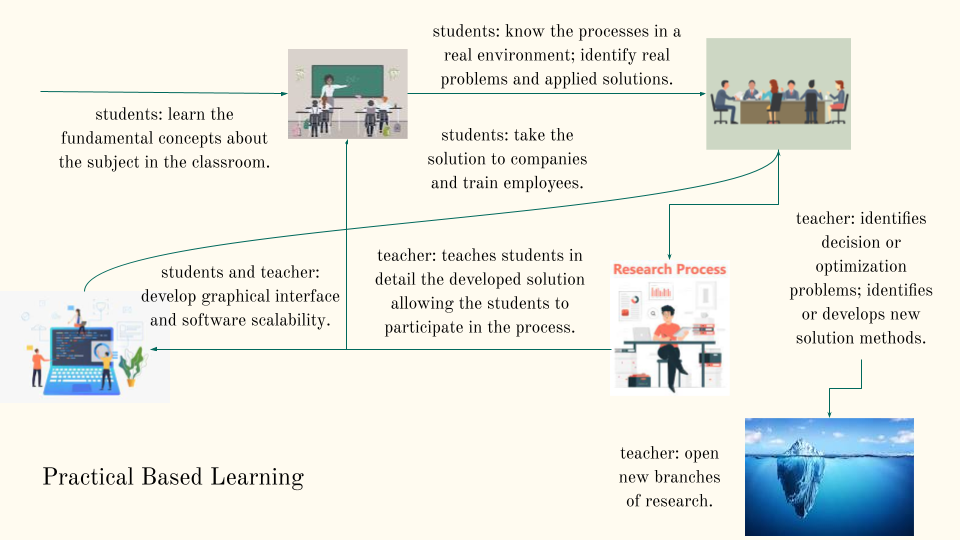
\includegraphics[width=\textwidth]{figures/graphicalAbstract.png}
\end{graphicalabstract}

%%Research highlights
\begin{highlights}
\item This paper presents a strategy for teaching undergraduate students based on practical experience
\item This strategy is strongly associated with the inseparability between teaching, research, extension and technological development
\item This paper also recommends some important resources that can be used to develop group work
\item And it discusses a solution to the impasse between transparency and guaranteeing the authenticity of the work, already widely used for software development but not in the development of research works
\end{highlights}

\begin{keyword}
%% keywords here, in the form: keyword \sep keyword
practical-based learning

%% PACS codes here, in the form: \PACS code \sep code

%% MSC codes here, in the form: \MSC code \sep code
%% or \MSC[2008] code \sep code (2000 is the default)

\end{keyword}

\end{frontmatter}

%% \linenumbers

%% main text

\section{Introduction}
\label{}

Problem-based learning (PBL) is a pedagogical approach applied worldwide, especially in nursing and medicine courses. 

\section{Practice-based learning}
\label{}

Practice-based learning strategy starts with students learning the basics of some science in the classroom. Concomitantly or after this first learning process, students carry out visits to an organization, through which they will be able to understand organizational processes, identifying aspects of the process that need to be better managed. Students then prepare a report of the visit, describing in detail the process studied and the real problems identified. Subsequently, this information is taken to the Teacher-Facilitator. Through discussions between the teacher and the students involved, the real problems, that is, the aspects of the studied process that need to be improved, are formatted as decision problems or optimization problems. And then a bibliographic survey is carried out on problems close to the identified problem and on methodologies that are applied in the solution of these first. Then a mathematical model and a solution algorithm are developed for the identified problem and the entire solution developed is passed on to the students, who in turn will take this knowledge to the company. Students will be responsible for carrying out tests to validate the developed solution and for training the company's employees.

For a better understanding of the difference between the real problem identified by the students and the formatted problem, consider the following example: after a student has visited a company that performs the maintenance service of hospital infusion pumps and analyzed in detail the processes of this company, she identified the following real problem:

\begin{quote}
"The company is unable to correctly program the hospital pump overhaul service. There are delays in maintenance and services are not prioritized correctly."
\end{quote}

After an in-depth study of the company's processes, and extensive discussions between teacher and student, it was identified that the problem was not associated with the maintenance process, but with the scheduling of equipment collection in hospitals, maintenance and return. In this context, a new allocation and routing problem was identified, defined as 'Problem of Planning the Maintenance and Transport of Hospital Infusion Pumps'. For more details on this issue see

Regarding the bibliographic survey, the teacher must identify the key words as well as what information should be sought in the consulted papers. Then, students will be able to participate in this survey, contributing to the identification of relevant works. Students should also be motivated to translate, read and understand at least one or two papers. 

Modeling can be completely performed by the teacher and then explained in detail to the students, or the teacher can explain the modeling process to the students along with some more complex constraints/functions, letting the students participate in this process. The development of the solution algorithm can also have the participation of students, as long as they have had previous training on programming or on the solution tool used (R, LINGO, MATLAB etc.). 

The developed SOLVER tests must be carried out with data from the studied company, collected by the students. It is important that students qualify company employees to use the SOLVER. Thus, the company will be able to take better advantage of the developed tool.


%% The Appendices part is started with the command \appendix;
%% appendix sections are then done as normal sections
%% \appendix

%% \section{}
%% \label{}

%% If you have bibdatabase file and want bibtex to generate the
%% bibitems, please use
%%
%%  \bibliographystyle{elsarticle-harv} 
%%  \bibliography{<your bibdatabase>}

%% else use the following coding to input the bibitems directly in the
%% TeX file.

\begin{thebibliography}{00}

%% \bibitem[Author(year)]{label}
%% Text of bibliographic item

\bibitem[ ()]{}

\end{thebibliography}
Donald E. Knuth (1986) \emph{The \TeX{} Book}, Addison-Wesley Professional.
\end{document}

\endinput
%%
%% End of file `elsarticle-template-harv.tex'.
